\documentclass[tikz, border=10pt]{standalone}
\usetikzlibrary{calc, automata, chains, arrows.meta, quotes}
\begin{document}
\tikzset{every loop/.style={min distance=10mm,in=120, out=60, looseness=10}}
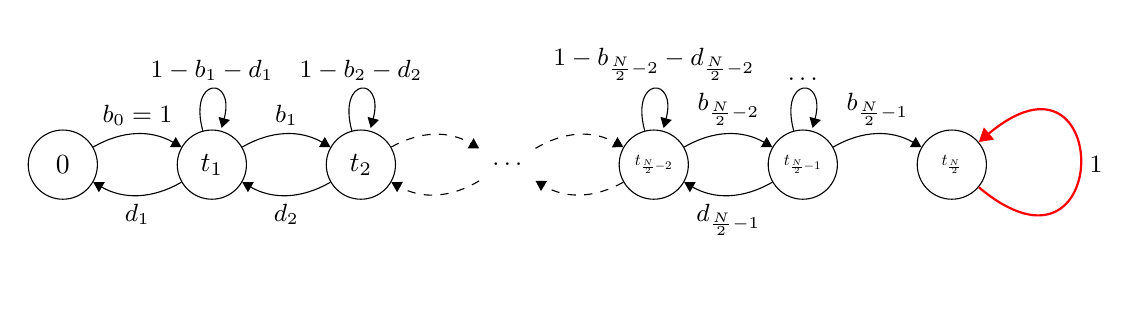
\begin{tikzpicture}[start chain = going right,
  -Triangle, every loop/.append style = {-Triangle}]
\node[state] (A) {$0$};
\node[state] (B) [right = of A] {$t_1$};
\node[state] (C) [right = of B] {$t_2$};
\node[state] (E) [right = of C, draw=none]  {$$}; % invisible node
\begin{small}
\draw (A) edge[bend left] node[above] {$b_0=1$} (B);
\draw (B) edge[bend left] node[below] {$d_1$} (A);
\draw (B) edge[bend left] node[above] {$b_1$} (C);
\draw (C) edge[bend left] node[below] {$d_2$} (B);
\draw (B) edge[loop above] node[above] {$1-b_1-d_1$} (B);
\draw (C) edge[loop above] node[above] {$1-b_2-d_2$} (C);

% \node[state] (D) [right = 2cm of C] {$3$};
\node[state] (D) [right = of C, draw=none] {$\ldots$}; % invisible node
\draw (C) edge[bend left, dashed] (D);
\draw (D) edge[bend left, dashed] (C);
                                % second part of the figure
%\node[state] (D1) [right = of C, draw=none] {$\ldots$}; % invisible node
\end{small}


\node[state] (A1) [right = of D]{\scalebox{0.6}{$t_{\frac{N}{2}-2}$}};
\node[state] (B1) [right = of A1] {\scalebox{0.6}{$t_{\frac{N}{2}-1}$}};

\node[state] (C1) [right = of B1] {\scalebox{0.6}{$t_{\frac{N}{2}}$}};


\draw (D) edge[bend left, dashed] (A1);
\draw (A1) edge[bend left, dashed] (D);

\begin{small}
\draw (A1) edge[bend left] node[above] {$b_{\frac{N}{2}-2}$} (B1);
\draw (B1) edge[bend left] node[below] {$d_{\frac{N}{2}-1}$} (A1);
\draw (B1) edge[bend left] node[above] {$b_{\frac{N}{2}-1}$} (C1);
%\draw (C1) edge[bend left] node[below] {$d_{\frac{N}{2}}$} (B1);
\draw (A1) edge[loop above] node[above] {$1-b_{\frac{N}{2}-2}-d_{\frac{N}{2}-2}$} (A1);
\draw (B1) edge[loop above] node[above] {$\ldots$} (B1);
\tikzset{every loop/.style={min distance=20mm,in=40, out=320, looseness=10}}
\draw (C1) edge[loop, thick, red] node[right, black] {$1$} (C1);
\end{small}
% \node[state] (D1) [right = 2cm of C] {$3$};
                                % just for arrow
\end{tikzpicture}
\end{document}
